% !TeX root = ../main.tex
\section{Цель работы}
\begin{itemize}
    \item Изучение принципа работы и получение практических навыков использования цифрового анализатора спектра;
    \item Изучение принципа работы и получение практических навыков использования генератора сигналов.
\end{itemize}

\begin{figure}[htbp]
    \centering
    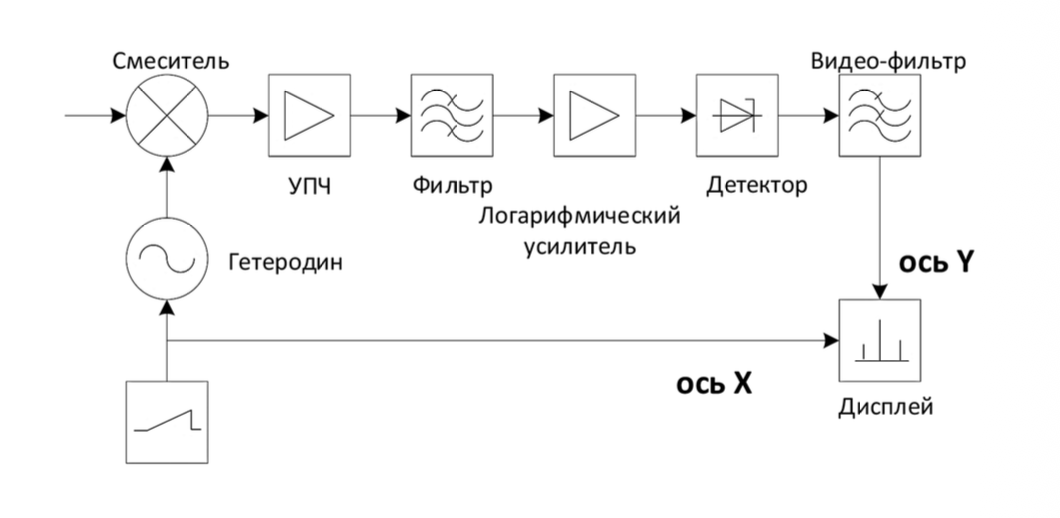
\includegraphics[width=0.9\linewidth]{Schema}
    \caption{Структурная схема анализатора спектра}
    \label{fig:spectrum_analyzer}
\end{figure}

Процесс формирования графического изображения на дисплее анализатора спектра, работающего по принципу супергетеродинного приемника, базируется на строгой синхронизации развертки по двум осям: оси частот (X) и оси амплитуд (Y).

В классических и многих современных архитектурах за развертку по оси X отвечает генератор пилообразного напряжения. Он формирует линейно нарастающее во времени напряжение $U_{sweep}(t)$, которое выполняет две синхронные функции:
\begin{itemize}
    \item \textbf{Управление гетеродином:} Перестраивает частоту локального генератора (гетеродина) $f_r(t)$ по линейному закону в пределах заданного диапазона обзора (Span).
    \item \textbf{Горизонтальная развертка:} Одновременно управляет отклонением луча (или координатой пикселя) по горизонтальной оси дисплея.
\end{itemize}
Математически развертку частоты можно выразить формулой:
\begin{equation}
    f_r(t) = f_{start} + \frac{f_{span}}{T_{sweep}} \cdot t
\end{equation}
где $T_{sweep}$ --- время развертки (Sweep Time). Таким образом, каждая точка на оси X на экране жестко привязана к определенной частоте входного сигнала в данный момент времени.

\subsection*{Формирование оси Y (Амплитуда)}
Вертикальное отклонение на экране формируется из амплитуды сигнала, прошедшего сложный путь обработки в радиотракте:
\begin{itemize}
    \item \textbf{Преобразование частоты:} Входной сигнал смешивается с перестраиваемым сигналом гетеродина. Полезные комбинационные составляющие попадают в тракт промежуточной частоты (ПЧ).
    \item \textbf{Фильтрация (RBW):} Сигнал проходит через узкополосный фильтр разрешения (RBW), который выделяет конкретную спектральную составляющую.
    \item \textbf{Логарифмирование:} Логарифмический усилитель сжимает огромный динамический диапазон амплитуд в удобный для восприятия логарифмический масштаб (выраженный в дБм).
    \item \textbf{Детектирование и сглаживание:} Детектор выделяет огибающую сигнала, а видео-фильтр (VBW) очищает ее от высокочастотных шумов.
\end{itemize}
Координата Y на экране пропорциональна логарифмическому уровню мощности выделенного сигнала:
\begin{equation}
    Y(t) \propto 10 \cdot \log_{10} \left( \frac{P_{det}(t)}{1 \text{ мВт}} \right)
\end{equation}

\subsection*{Форма отображаемого спектрального пика}
Ключевая особенность формирования изображения в супергетеродинном анализаторе заключается в том, что идеальный гармонический (синусоидальный) сигнал отображается не в виде бесконечно тонкой дискретной линии, а в виде колоколообразного пика. 

Это происходит потому, что при плавной перестройке частоты гетеродина спектральная линия входного сигнала <<протаскивается>> через фильтр ПЧ. В результате форма пика, который рисуется на дисплее, является точным графическим отображением амплитудно-частотной характеристики (АЧХ) самого фильтра RBW. 

В современных приборах АЧХ фильтров разрешения проектируется так, чтобы иметь форму, близкую к гауссовой кривой, что минимизирует переходные процессы при быстрой развертке:
\begin{equation}
    H(f) \approx \exp\left( - \frac{(f - f_c)^2}{2\sigma^2} \right)
\end{equation}
Именно поэтому уменьшение полосы RBW (значения $\sigma$) делает пики на экране более острыми, приближая их к теоретическому виду дискретного спектра, и одновременно снижает средний отображаемый уровень шума (DANL).
